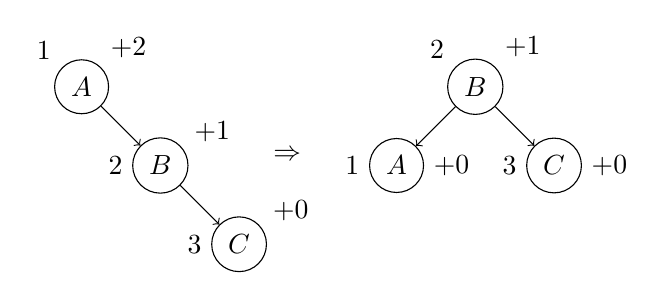
\begin{tikzpicture}[->, auto]
        \tikzstyle{vertex} = [circle,draw=black]
        \node[vertex, label = {140: $1$} , label = {45: $+2$} ] (1) at (0,0) {$A$};   
        \node[vertex, label = {180: $2$} , label = {30: $+1$}] (2) at (1, -1) {$B$};
        \node[label={above:$\Rightarrow$},rotate=45] at (3,-1.15) {};
        \node[vertex, label = {180: $3$}, label = {30: $+0$}] (3) at (2,-2) {$C$};
        \node[vertex, label = {140: $2$} , label = {45: $+1$} ] (4) at (5,0) {$B$};   
        \node[vertex, label = {180: $1$} , label = {0: $+0$}] (5) at (4, -1) {$A$};
        \node[vertex, label = {180: $3$}, label = {0: $+0$}] (6) at (6,-1) {$C$};
        \path   
                (1) edge (2)
                (2) edge (3)
                (4) edge (5)
                (4) edge (6);
\end{tikzpicture}